\section{Inductive Sets and Relations}
\label{setrelation}

\subsection{Inductive Sets}

\paragraph{Set Notation}

A set is an unordered collection of objects. If the object $a$ is an element of the set
$A$ we write $a \in A$.

A set $A$ is a subset of set $B$ if all elements of the set $A$ are also
elements of the set $B$. The symbol $\subseteq$ is used to express the subset
relation. The operator $:=$ is used to express that something is valid by
definition. Therefore the subset relation is defined symbolically by
$A \subseteq B := \forall a\mathbin. a \in A \imp a \in B$. The statement
$A \subseteq B$ can always be replaced by its definition
$\forall a\mathbin. a \in A \imp a \in B$ and vice versa.

The double arrow $\imp$ is used to express implication. $p \imp q$ states the
assertion that having a proof of $p$ we can conclude $q$. The assertion $p
\imp q$ is proved by assuming $p$ and deriving the validity of $q$.




\paragraph{Rule Notation}

We have often several premises which are needed reach a conclusion. E.g. we
might have the assertion $p_1 \land p_2 \land \ldots \imp c$. Then we use the
rule notation $\ruleh{p_1, p_2, \ldots}{c}$ or $\rulev{p_1 \\ p_2\\
  \vdots}{c}$ to express the same fact. Evidently the order of the premises is
not important.

Variable in rules are universally quantified. Therefore we can state the
subset definition $\forall a\mathbin. a \in A \imp a \in B$. in rule notation more
compactly and better readable as $\ruleh{a \in A}{a \in B}$. It should be clear
from the context which symbols denote variables.


\paragraph{Inductive Definition of Sets}

Rules can be used to define sets inductively. The set of even numbers $E$ can be
defined by the two rules $0 \in E$ and $\ruleh {n \in E}{n+2 \in E}$. A set
defined by rules is the least set which satisfies the rules. The set $E$ of
even number must contain the number $0$ and with all numbers $n$ it contains
also the number $n+2$.

The fact that some object is an element of an inductively defined set must be
established by an arbitrarily long but finite sequence of applications of the
rules which define the set. A proof of $4 \in E$ consists of a proof of $0 \in
E$ by application of the first rule and then two applications of the second
rule to reach $2 \in E$ and $4 \in E$.






\paragraph{Rule Induction}

If we have the fact that an object is an element of some inductively defined
set then we can be sure that it is in the set because of one of the rules
which define the set.

This can be used to prove facts by rule induction. Suppose we want to prove
that some property $p$ is shared by all even numbers. We can express this
statement by the rule $\ruleh {n \in E}{p(n)}$. Note that variables in rules
are implicitly universally quantified, i.e. the rule expresses the statement
$\forall n \mathbin. n \in E \imp p(n)$.

It is possible to prove this statement by induction on $n \in E$. Such a proof
consists of a proof of the statement for each rule. In the case of even
numbers there are two rules.

For the first rule we have to prove the the number $0$ satisfies the property
$p(0)$.

For the second rule we assume that $n \in E$ because there is some other
number $m$ already in the set of even numbers $E$ and $n = m+2$. I.e. we have
to prove the goal $p(m+2)$ under the premise $m \in E$. Because of the premise
$m \in E$ we can assume the induction hypothesis $p(m)$. I.e. we can assume
$m \in E$ and $p(m)$ and derive the validity of $p(m+2)$.

If the proof succeeds for both rules we are allowed to conclude that the
property $p$ is satisfied by all even numbers.



\paragraph{Natural Number Induction}

It is not difficult to see that the usual law of induction on natural numbers
is just a special case of rule induction. We can define the set of natural
numbers inductively $\mathbb{N}$ by the rules
\begin{enumerate}
\item $0 \in \mathbb{N}$
\item $\ruleh{n \in \mathbb{N}} {n' \in \mathbb{N}}$
\end{enumerate}
where $n'$ denotes the successor of $n$ i.e. $3$ is just a shorthand for
$0'''$.

The usual induction law of natural numbers allows to prove a property $p$ for
all natural number by a proof of $p(0)$ and a proof of
$\forall n\mathbin. p(n) \imp p(n')$ which are exactly the requirements of a
proof by rule induction.





\paragraph{Grammar Notation}

In some cases it is convenient to define a set by a grammar. E.g. we can
define the set of natural numbers by all terms $n$ generated by the grammar
%
    $$ n ::= 0 \mid n'$$
%
i.e. we can use the corresponding induction law to prove
that all terms generated by the grammar satisfy a certain property.

This definition is just a special form of the definition of the set of natural
numbers $\mathbb{N}$ by the rules
\begin{enumerate}
\item $0 \in \mathbb{N}$
\item $\ruleh{n \in \mathbb{N}} {n' \in \mathbb{N}}$
\end{enumerate}





\subsection{Inductive Relations}


\paragraph{Relations}

n-ary relations are just sets of n-tuples. A binary relation $r$ over the sets
$A$ and $B$ is a subset of the cartesian product
$$
    r \subseteq A \times B.
$$ We use the notations $(a,b) \in r$, $r(a,b)$ and $a \to_r b$ to denote the
fact that the pair $(a,b)$ with $a \in A$ and $b \in B$ figure in the relation
$r$.

In this paper we need only endorelations i.e. binary relations where the
domain $A$ and the range $B$ of the relation are the same set.




\paragraph{Relation Closure}

As with sets, relations can be defined inductively.


% Transitive Closure
% --------------
\begin{definition} The \emph{transitive closure} $\rplus{r}$ of a relation $r$ is
  defined by the rules
  \begin{enumerate}
  \item $\ruleh {r(a,b)} {\rplus{r}(a,b)}$
  \item $\ruleh{\rplus{r}(a,b),\, r(b,c)}{\rplus{r}(a,c)}$
  \end{enumerate}
\end{definition}

The rules can be displayed graphically. The premises are marked blue and the
conclusion is marked red.

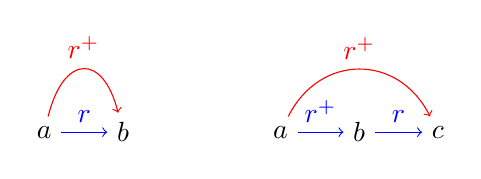
\begin{tikzpicture}
  \node (a0) at (0,0) {$a$};
  \node (b0) at (1,0) {$b$};

  \node (a) at (3,0) {$a$};
  \node (b) at (4,0) {$b$};
  \node (c) at (5,0) {$c$};

  \draw [->,blue] (a0) edge node[above]{$r$} (b0);
  \draw [->,red]   (a0) .. controls (0.25,1) and (0.75,1) .. node[above] {$r^+$} (b0);

  \path[->,blue] (a) edge node[above] {$r^+$} (b);
  \path[->,blue] (b) edge node[above] {$r$}    (c);
  \draw[->,red]   (a) .. controls (3.5,1) and (4.5,1) ..  node[above] {$r^+$}    (c);
\end{tikzpicture}


We called $r^+$ the transitive closure of $r$, but the fact that $r^+$ is
transitive needs a proof.

\begin{theorem}
  \label{plustransitive}
  The transitive closure $r^+$ of the relation $r$ is transitive
  i.e. $\ruleh{a \to_r^+ b, \, b \to_r^+ c} {a \to_r^+ c}$ is valid.
  \begin{proof}
    Assume $a \to_r^+ b$ and prove the goal $a \to_r^+ c$ by induction on
    $b \to_r^+ c$.
    \begin{enumerate}
    \item
      Goal $a \to_r^+ c$ assuming $b \to_r^+ c$ and that
      $b \to_r^+ c$ is valid by rule 1 of the transitive closure.\\
      Premise $b \to_r c$.\\
      The goal is valid by the assumption $a \to_r^+ b$, the premise $b \to_r
      c$ and rule 2 of the transitive closure.

    \item
      Goal $a \to_r^+d$ assuming $b \to_r^+ d$ and that
      $b \to_r^+ d$ is valid by rule 2 of the transitive closure. \\
      Premises $b \to_r^+ c$ and $c \to_r d$.\\
      Induction hypothesis $a \to_r^+ c$.\\
      The goal is valid by the induction hypothesis $a \to_r^+ c$, the premise
      $c \to_r d$ and rule 2 of the transitive closure.
    \end{enumerate}
  \end{proof}
\end{theorem}




% Reflexive Transitive Closure
% ----------------------
\begin{definition} The \emph{reflexive transitive closure} $\rstar{r}$ of a relation $r$ is
  defined by the rules
  \begin{enumerate}
  \item $\rstar{r}(a,a)$
  \item $\ruleh{\rstar{r}(a,b), \, r(b,c)}{\rstar{r}(a,c)}$
  \end{enumerate}
\end{definition}

Graphical representation of the rules:

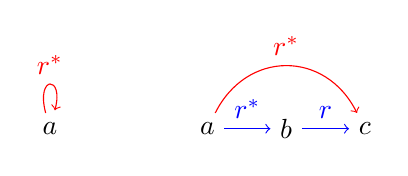
\begin{tikzpicture}
  \node (reflexive) at (0,0) {$a$};
  \node (a) at (2,0) {$a$};
  \node (b) at (3,0) {$b$};
  \node (c) at (4,0) {$c$};

  \path (reflexive) edge [loop above,red] node {$r^*$} (reflexive);

  \path[->,blue] (a) edge node[above] {$r^*$} (b);
  \path[->,blue] (b) edge node[above] {$r$}    (c);
  \draw[->,red]   (a) .. controls (2.5,1) and (3.5,1) ..  node[above] {$r^*$}    (c);
\end{tikzpicture}

\begin{theorem}
  \label{startranstive}
  The reflexive transitive closure $r^*$ of the relation $r$ is transitive
  i.e. $\ruleh{a \to_r^* b, \, b \to_r^* c} {a \to_r^* c}$ is valid.
  Proof similar to the proof of theorem~\ref{plustransitive}.
\end{theorem}




% Equivalence Closure
% ----------------
\begin{definition}
  \label{def:equivalenceclosure}
  The \emph{equivalence closure} $\reqv{r}$ of a relation $r$ is
  defined by the rules
  \begin{enumerate}
  \item
    $\reqv{r}(a,a)$
  \item
    $\ruleh{
      \reqv{r}(a,b), \,   r(b,c)}
    {\reqv{r}(a,c)}$
  \item
    $\ruleh{\reqv{r}(a,b), \, r(c,b)} {\reqv{r}(a,c)}$
  \end{enumerate}
\end{definition}

Again a graphical representation of the rules:

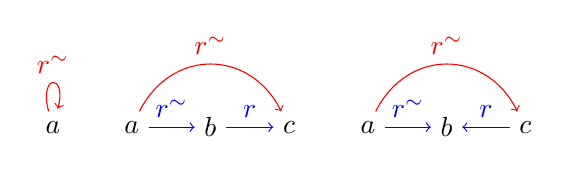
\begin{tikzpicture}
  \node (a0) at (0,0) {$a$};
  \path (a0) edge [loop above,red] node {$r^\sim$} (a0);

  \node (a1) at (1,0) {$a$};
  \node (b1) at (2,0) {$b$};
  \node (c1) at (3,0) {$c$};
  \draw[->,blue] (a1) edge node[above]{$r^\sim$} (b1);
  \draw[->,blue] (b1) edge node[above]{$r$} (c1);
  \draw[->,red] (a1) .. controls (1.5,1) and (2.5,1) .. node [above]{$r^\sim$} (c1);

  \node (a2) at (4,0) {$a$};
  \node (b2) at (5,0) {$b$};
  \node (c2) at (6,0) {$c$};
  \draw[->,blue] (a2) edge node[above]{$r^\sim$} (b2);
  \draw[<-,blue] (b2) edge node[above]{$r$} (c2);
  \draw[->,red]   (a2) .. controls (4.5,1) and (5.5,1) .. node [above]{$r^\sim$} (c2);
\end{tikzpicture}

\begin{theorem}
  \label{eqvtransitive}
  The equivalence closure is transitive. Proof similar to the proof of
  theorem~\ref{plustransitive}.
\end{theorem}

\begin{theorem}
  The equivalence closure is symmetric i.e. $\ruleh {a \to_r^\sim b} {b
    \to_r^\sim a}$.
  \begin{proof}
    We proof this theorem in 3 steps. First we proof two lemmas and then the
    theorem by induction.
    \begin{itemize}
    \item Lemma 1: $\ruleh{a \to_r b}{a \to_r^\sim b}$. Proof. Assume $a \to_r
      b$. We get $a \to_r^\sim a$ by rule 1 and then $a \to_r^\sim b$ by the
      assumption and rule 2.
    \item
      Lemma 2: $\ruleh{a \to_r b}{b \to_r^\sim a}$. Proof. Assume $a \to_r b$.
      We get $b \to_r^\sim b$ by rule 1 and then $b \to_r^\sim a$ by the
      assumption and rule 3.
    \item
      $\ruleh {a \to_r^\sim b} {b \to_r^\sim a}$ by induction on
      $a \to_r^\sim b$.
      \begin{enumerate}
      \item
        Goal $a \to_r^\sim a$. Trivial by reflexivity.

      \item
        Goal $c \to_r^\sim a$ assuming that $a \to_r^\sim c$ is valid by rule 2 of
        the equivalence closure.\\
        Premises $a\to_r^\sim b$ and $b \to_r c$.\\
        Induction hypothesis $b \to_r^\sim a$.\\
        We get $c \to_r^\sim b$ by the second premise and lemma 2 and then $c
        \to_r^\sim a$ by the induction hypothesis and transitivity of the
        equivalence closure~\ref{eqvtransitive}.

      \item
        Goal $c \to_r^\sim a$ assuming that $a \to_r^\sim c$ is valid by rule 3 of
        the equivalence closure.\\
        Premises $a\to_r^\sim b$ and $c \to_r b$.\\
        Induction hypothesis $b \to_r^\sim a$.\\
        We get $c \to_r^\sim b$ by the second premise and lemma 1 and then $c
        \to_r^\sim a$ by the induction hypothesis and transitivity of the
        equivalence closure~\ref{eqvtransitive}.

      \end{enumerate}
    \end{itemize}
  \end{proof}
\end{theorem}



% Closures are increasing, monotonic and idempotent
% -----------------------------------------
\begin{theorem}
  All closures are increasing $r \subseteq r^c$, monotonic
  $r \subseteq s \imp r^c \subseteq s^c$ and idempotent $r^{cc} = r^c$ (where
  the superscript $c$ stands for $+$, $*$ or $\sim$).
  \begin{proof}  We give a proof for the reflexive transitive closure. The
    proofs for the other closures are similar.
    \begin{itemize}
    \item
      Increasing: Goal $r(a,b) \imp \rstar{r}(a,b)$. By rule 1 we get
      $\rstar{r}(a,a)$. The assumption $r(a,b)$ and rule 2 imply
      $\rstar{r}(a,b)$.
      %
    \item
      Monotonic: Goal $\ruleh{r \subseteq s, \, \rstar{r}(a,b)}
      {\rstar{s}(a,b)}$. Prove by induction on $\rstar{r}(a,b)$.
        \begin{enumerate}
        \item Case $a=b$. Goal $s^*(a,a)$. Trivial by reflexivity of $\rstar{s}$.
        \item
          Goal $s^*(a,c)$ assuming $r\subseteq s$ and $r^*(a,c)$ is valid
          because of rule 2. Premises $r^*(a,b)$ and $r(b,c)$. Induction
          hypothesis $s^*(a,b)$.
          \\
          $
          \begin{matrix}
            a  & \to_{\rstar{r}} & b   &  \to_r   & c \\
                &    \Downarrow_1 & &  \Downarrow_2\\
            a  & \to_{\rstar{s}} & b   &  \to_s  &  c
          \end{matrix}$.\\
          $\Downarrow_1$ is valid by the induction
          hypothesis. $\Downarrow_2$ is valid by $r \subseteq s$. From the
          last line and the rule 2 of the reflexive transitive closure we can
          conclude $\rstar{s}(a,c)$.
        \end{enumerate}
    \item
      Idempotent: The equality of the relations $r^{**} = r^*$ needs a proof
      of $r^{**} \subseteq r^*$ and a proof of $r^* \subseteq r^{**}$.
      \begin{itemize}
      \item $ r^* \subseteq r^{**}$ is valid because the
        closure is increasing.
      \item
        Goal $\ruleh{r^{**}(a,b)} {r^*(a,b)}$. Proof by induction on $r^{**}(a,b)$.
        \begin{enumerate}
        \item
          Case $a=b$. Goal $r^*(a,a)$. Trivial by reflexivity.
        \item
          Goal $r^*(a,c)$ assuming $r^{**}(a,c)$ is valid because of rule 2.
          Premises $r^{**}(a,b)$ and $r^*(b,c)$. Induction
          hypothesis $r^*(a,b)$.
          $
          \begin{matrix}
            a  & \to_{r^{**}} & b   &  \to_{r^*}   & c \\
                &    \Downarrow_1 & &  \Downarrow_2\\
            a  & \to_{r^*} & b   &     \to_{r^*}   &  c
          \end{matrix}$.
          $\Downarrow_1$ is valid by the induction
          hypothesis. $\Downarrow_2$ is trivial. $r^*$ is
          transitive. Therefore the last line implies $r^*(a,c)$.
        \end{enumerate}
      \end{itemize}
    \end{itemize}
  \end{proof}
\end{theorem}






\begin{theorem}
  \label{sameclosure}
A relation $s$ which satisfies $r \subseteq s \subseteq r^c$ has the same closure
as $r$ i.e. $r^c = s^c$. Proof:
  \begin{itemize}
  \item $r^c \subseteq s^c$ by monotonicity.
  \item $s^c \subseteq r^c$: $s^c \subseteq r^{cc}$ by
    monotonicity and then use idempotence to conclude $s^c \subseteq r^c$.
  \end{itemize}
\end{theorem}





\paragraph{Terminal Elements}

\begin{definition}
  The set of \emph{terminal elements} $T_r$ of the relation $r$ is
  defined by the rule
  $$
  \ruleh{
    \begin{bmatrix}
      \ruleh {a\to b} {\perp}
    \end{bmatrix}}
  {a \in T_r}$$
%
  where $\perp$ is used to denote a contradiction and the square brackets $[$
  and $]$ around the rule above the line indicate that the variables not used
  outside the bracketed rule are universally quantified in the inner
  rule. I.e. in order to establish $a \in T_r$ we have to prove
  $\forall b \mathbin. \neglow a \to_r b$ or
  $\forall b\mathbin. a \to_r b \imp \perp$.
%
  Note that the scope of the universal quantification of the variable $a$
  spans the whole rule while the scope of the universal quantification of the
  variable $b$ is just the premise of the rule (i.e. the part above the line).
\end{definition}



\begin{theorem}
  \label{trivialpaths}
  A terminal element $a$ of a relation $r$ has only trivial outgoing paths:
  $\ruleh {a \in T_r, \, a \to_r^* b} {a = b}$.
  \begin{proof} By induction on $a \to_r^* b$.
    \begin{enumerate}
    \item
      Goal $a = a$. Trivial.
    \item
      Goal $a = c$ assuming that $a \to_r^* c$ is valid by rule 2. Premises
      $r^*(a,b)$ and $r(b,c)$. Induction hypothesis $a = b$. Therefore the
      second premise states $r(a,c)$ which contradicts the assumption $a \in T_r$.
    \end{enumerate}
  \end{proof}
\end{theorem}




\paragraph{Weakly Terminating Elements}

\begin{definition}
  $a$ is a \emph{(weakly) terminating element} of the relation $r$ if there
  is a path to a terminal element $b$ i.e. $a \to_r^* b$. The set of
  \emph{weakly terminating elements} $WT_r$ of the relation $r$ is defined by
  the rule $\ruleh{a \to_r^* b, \, b \in T_r} {a \in WT_r}$.
\end{definition}






\paragraph{Strongly Terminating Elements}

\begin{definition}
  An object $a$ is \emph{strongly terminating} with respect to the relation
  $r$ if all paths from $a$ end at some terminal element of $r$. We define the
  set of strongly terminating elements $ST_r$ of the relation $r$ by the rule
%
$$
   \ruleh
   {
     \begin{bmatrix}
       \ruleh {a \to_r b} {b \in ST_r}
     \end{bmatrix}
   }
   {a \in ST_r}
$$
\end{definition}

This definition might need some explanation to be understood correctly. Since
the premise of the rule is within brackets, all variables not occuring outside
the brackets are universally quantified within the brackets (here the variable
$b$).

The rule says that all objects $a$ where all successors $b$ with respect to
the relation are strongly terminating are strongly terminating as well. The
rule is trivially satisfied by all objects which have no successors i.e. all
terminal objects. If the relation $r$ has no terminal objects then there
are no initial objects which are strongly terminating.

If there are terminal elements then step by step strongly terminating objects
can be constructed by the rule that all successors of them must be strongly
terminating (or already terminal). For each constructed strongly terminating
object it is guaranteed that all paths starting from it must end within a finite
number of steps at some terminal object of the relation.




An object $a$ without successors with respect to the relation $r$ i.e. if
there are no $b$ with $a \to_r b$ satisfy the rule, because the premise is
satified vacuously. An object $a$ without successors is a terminal element by
definition. I.e. all terminal elements are strongly terminating.










\subsection{Diamonds and Confluence}
\label{sec:diamondsconfluence}

In this section we define diamonds and confluent relations.

A relation is called confluent if starting from some object following the
relation on different paths of arbitrary length there is always some other
object where the two paths meet. This intuitive definition is made precise in
the following.

A diamond relation is a kind of a confluent relation where one step different
paths can join withing one step.

It turns out that confluence is a rather strong property of a relation. It
guarantees that
\begin{itemize}
\item all equivalent elements meet at some point
\item all paths to terminal elements end up at the same terminal
  element (i.e. terminal elements are unique)
\end{itemize}

A diamond relation is a superset of a confluent relation which has already the
essential part of confluence. It turns out that a diamond relation is confluent.

First we define formally the diamond property of a relation. The diamond
property is intuitively a one step confluence.

\begin{definition}
A relation $r$ is a \emph{diamond} if for all $a$, $b$ and $c$ there exists a $d$
such that
$
  \begin{matrix}
    a & \to_r & b \\
    \downarrow_r & & \downarrow_r \\
    c & \to_r & \exists d
  \end{matrix}
$ holds.
\end{definition}

\noindent Note that we use the picture
$$\begin{matrix}
  a & \to_r & b \\
  \downarrow_r & & \downarrow_r \\
  c & \to_r & \exists d
\end{matrix}$$ to express the statement
$$\ruleh {a \to_r b, \, a \to_r c} {\exists d\mathbin. b\to_r d \land c\to_r
  d}.$$
%
The picture notation is more intuitive but not less precise because it can be
translated into the corresponding rule notation which can be translated
uniquely into a statement of predicate logic.

\begin{definition}
  A relation $r$ is \emph{confluent} if $\rstar{r}$ is a diamond.
\end{definition}

\begin{theorem} In a confluent relation $r$ all two $r$-equivalent elements
  meet at some common element in zero or more steps
  $
  \begin{matrix}
    a & \to_r^\sim & b \\
    & \searrow_r^* & \downarrow_r^*\\
    & & \exists c
  \end{matrix}
  $.
  \begin{proof}
    By induction on $a \to_r^\sim b$.
    \begin{enumerate}

    \item $a = b$. Trivial. Take $c = a$.

    \item
      Goal
      $\begin{matrix}
        a    & \to_r^\sim      & c                      \\
              & \searrow_r^* & \downarrow_r^*  \\
        & & \exists e
      \end{matrix}$
      where $a \to_r^\sim c$ is valid by rule 2. Premises $a \to_r^\sim b$
      and $b \to_r c$.
      Induction hypothesis
      $\begin{matrix}
        a    & \to_r^\sim      & b                      \\
              & \searrow_r^* & \downarrow_*  \\
        & & \exists d
      \end{matrix}$.\\
      Proof
      $\begin{matrix}
        a & \reqv\to & b & \to_r & c\\
        & \searrow_r^* & \downarrow_r^*  & & \downarrow_r^*\\
        & & \exists d & \to_r^* & \exists e
      \end{matrix}$.
      $d$ exists by induction hypothesis, $e$ exists by confluence.

    \item
      Goal
      $\begin{matrix}
        a    & \to_r^\sim      & c                      \\
              & \searrow_r^* & \downarrow_r^*  \\
        & & \exists e
      \end{matrix}$
      where $a \to_r^\sim c$ is valid by rule 3. Premises $a \to_r^\sim b$
      and $b \gets_r c$.
      Induction hypothesis
      $\begin{matrix}
        a    & \to_r^\sim      & b                      \\
              & \searrow_r^* & \downarrow_r^*  \\
        & & \exists d
      \end{matrix}$.\\
      Proof
      $\begin{matrix}
        a & \reqv\to & b & \gets_r & c\\
        & \searrow_r^* & \downarrow_r^*  & & \downarrow_r^*\\
        & & \exists d & \to_r^* & \exists e
      \end{matrix}$.
      $d$ exists by induction hypothesis, $e$ exists by confluence.
    \end{enumerate}
  \end{proof}
\end{theorem}


\begin{theorem}
  In a confluent relation all paths from the same object ending at some terminal
  object end at the same terminal object, i.e.
  $$\ruleh {a \to_r^* b, \, a \to_r^* c, \, b \in T_r, \, c \in T_r} {b = c}$$.

  \begin{proof}
    Suppose there are two terminal elements $b$ and $c$ with paths starting
    from the object $a$.
    By definition of confluence there must be a $d$ such that
    $\begin{matrix} a & \tostar & b \\
      \downarrow_* & & \downarrow_* \\
      c & \tostar & d
    \end{matrix}$ is valid. Since $b$ and $c$ are terminal objects by
    theorem~\ref{trivialpaths} there are only trivial outgoing paths from $b$
    and $c$ which implies that $b = c = d$ must be valid.
  \end{proof}
\end{theorem}


\begin{theorem}
  \label{th:diamondconfluent}
  A diamond relation is confluent.
  \begin{proof}
    We prove this theorem in two steps.
    \begin{itemize}
    \item Lemma: Let $r$ be a diamond. Then
      $\begin{matrix}
        a                     &    \to_r^*    &    b \\
        \downarrow_r &                   & \downarrow_r \\
        c                     & \to_r^*       & \exists d
      \end{matrix}$ is valid.
      Proof by induction on $a \to_r^* b$.
      \begin{enumerate}
      \item
        Case $a = b$. Trivial, take $d=c$.
      \item
        Goal $\begin{matrix}
          a                     &    \to_r^*    &    c \\
          \downarrow_r &                   & \downarrow_r \\
          d                     & \to_r^*       & \exists f
        \end{matrix}$ where $a \to_r^* c$ is valid because of rule 2.
        Premises $a \to_r^* b$ and $b \to_r c$.
        Induction hypothesis
        $\begin{matrix}
          a                     &    \to_r^*    &    b \\
          \downarrow_r &                   & \downarrow_r \\
          d                     & \to_r^*       & \exists e
        \end{matrix}$.
        \\
        Proof:
        $\begin{matrix}
          a                     & \to_r^* & b                     & \to_r & c\\
          \downarrow_r &             & \downarrow_r &          & \downarrow_r\\
          d                     & \to_r^* & \exists e        & \to_r & \exists f
        \end{matrix}$. $e$ exists by the induction hypothesis, $f$ exists because
        $\to_r$ is a diamond.
      \end{enumerate}

    \item Theorem:  Let $r$ be a diamond. Then
      $\begin{matrix}
        a                     & \to_r^*     & b \\
        \downarrow_r^* &                 & \downarrow_r^* \\
        c                        & \to_r^*     & \exists d
      \end{matrix}$ is valid.
      Proof by induction on $a \to_r^* c$.
      \begin{enumerate}
      \item
        Case $a = b$. Trivial, take $d=c$.
      \item
        Goal
        $\begin{matrix}
          a                     & \to_r^*     & b \\
          \downarrow_r^* &                 & \downarrow_r^* \\
          d                        & \to_r^*     & \exists f
        \end{matrix}$ where $a \to_r^* d$ is valid because of rule 2.
        Premises $a \to_r^* c$ and $c \to_r d$.
        Induction hypothesis
        $\begin{matrix}
          a                     & \to_r^*     & b \\
          \downarrow_r^* &                 & \downarrow_r^* \\
          c                        & \to_r^*     & \exists e
        \end{matrix}$.
        \\
        Proof
        $\begin{matrix}
          a                        & \to_r^*  & b\\
          \downarrow_r^* &              & \downarrow_r^* \\
          c                        & \to_r^*  & \exists e  \\
          \downarrow_r    &              & \downarrow_r \\
          d                        & \to_r^*  & \exists f
        \end{matrix}$.
        $e$ exists by induction hypothesis, $f$ exists by the previous lemma.
      \end{enumerate}
    \end{itemize}
  \end{proof}
\end{theorem}

The last theorem stating that diamonds are confluent gives a way to prove that
a relation $r$ is confluent. If $r$ is already a diamond we are ready since a
diamond is confluent. If $r$ is not a diamond we try to find a diamond
relation $s$ between $r$ and its reflexive transitive closure $r^*$ i.e. a
relation $s$ which satisfies $r \subseteq s \subseteq r^*$. From the
theorem~\ref{sameclosure} we know that $s$ and $r$ have the same reflexive
transitive closure i.e. $r^* = s^*$. Since $s$ is a diamond, $s^*$ is a
diamond as well and therefore $r$ is confluent.

In order to find a diamond relation $s$ we can search for rules which are
satisfied by $r^*$ and are intuitively the reason which let us assume that $r$
is confluent. Then we can define $s$ inductively as the least relation
satisfying the rules and hope that we can prove that $s$ is a diamond with $r
\subseteq s$. Note that $s \subseteq r^*$ is satisfied implicitly by this
approach since $r^*$ satisfies the rules and $s$ is the least relation
satisfying the rules.
